\documentclass[11pt]{beamer}

\usepackage[utf8]{inputenc}
\usepackage[T1]{fontenc}
\usepackage{lmodern}
\usepackage[french]{babel}
\usetheme{Copenhagen}
%\usecolortheme{beaver}
\useoutertheme{split} % ???
\usefonttheme{serif}

\setbeamertemplate{theorems}[numbered] % to number

% Formules mathématiques
\usepackage{amsmath}
\usepackage{amsfonts}
\usepackage{amssymb}
\usepackage{amsthm}
\usepackage{nicefrac}
\usepackage{mathrsfs}

\usepackage{tikz}
\usetikzlibrary{arrows.meta}
\usepackage[linguistics]{forest}
\usepackage{graphicx}
\graphicspath{ {../simulation/figures/}}
\usepackage{xcolor}

\begin{document}
	\author{Hugo \textit{Vangi}lluwen}
	\title{Probabilité des critères de vote}
	\subtitle{TIPE}
	%\logo{}
	%\institute{}
	\date{\today}
	\subject{Systèmes de vote}
	%\setbeamercovered{transparent}
	%\setbeamertemplate{navigation symbols}{}
	
	\begin{frame}[plain]
		\maketitle
	\end{frame}
	
	\begin{frame}
		\small \tableofcontents % [hideallsubsections]
	\end{frame}
	
	\AtBeginSection{
		\begin{frame}
			\small \tableofcontents[currentsection]
		\end{frame}
	}
	
	\section{Différents systèmes de vote}
	
	\subsection{Exemple introductif}
	\begin{frame}{Exemple introductif}
		\uncover<2-4>{
			\small
			\textbf<2>{Scrutin Uninominal}
			\
			\textbf<3>{Méthode de Borda}
			\
			\textbf<4>{Scrutin de Condorcet}
		}
		\begin{exampleblock}{Exemple}
			\begin{tabular}{ccccccc}
				5 &:& A &>& B &>& C \\
				6 &:& C &>& B &>& A \\
				2 &:& B &>& A &>& C \\
			\end{tabular}
			\uncover<2-4>{
				\newline
				\alt<2-3>{
					\begin{tabular}{ccccccccc}
						\alt<2>{
							A &:& 5*1 &+& 6*0 &+& 2*0 &=& 5 \\
							B &:& 5*0 &+& 6*0 &+& 2*1 &=& 2 \\
							C &:& 5*0 &+& 6*1 &+& 2*0 &=& 6 \\
							Résultat &:& C > A > B
						}{
							A &:& 5*2 &+& 6*0 &+& 2*1 &=& 12 \\
							B &:& 5*1 &+& 6*1 &+& 2*2 &=& 15 \\
							C &:& 5*0 &+& 6*2 &+& 2*0 &=& 12 \\
							Résultat &:& B > C = A
						}
					\end{tabular}
					}{
						\begin{figure}
							\centering
							\begin{tikzpicture}[
								node distance={30mm},
								thick,
								edge/.style = {draw, circle},
								arrow/.style={-{Stealth[length=4mm, width=3mm]}}
								]
								
								\node[edge] (A) {A};
								\node[edge] (B) [below left of=A] {B};
								\node[edge] (C) [below right of=A] {C};
								
								\draw[arrow] (B) -- node[midway, above, sloped] {3} (A);
								\draw[arrow] (B) -- node[midway, above, sloped] {1} (C);
								\draw[arrow] (A) -- node[midway, above, sloped] {1} (C);
							\end{tikzpicture}
						\end{figure}
					Résultat : B > A > C
					}
			}
		\end{exampleblock}
	\end{frame}
	
	\subsection{Théorie du choix social}
	\begin{frame}{Théorie du choix social}
		\begin{itemize}
			\item Étudie comment des opinions individuelles peuvent mener à une décision collective
			\item Domaine multidisciplinaire lié aux mathématiques (théorie de la décision), à l'économie, à la philosophie (politique), aux sciences humaines et sociales $\ldots$
		\end{itemize}
	\end{frame}
	
	\subsection{Choix du TIPE}
	\begin{frame}{Choix du TIPE}
		\begin{itemize}
			\item Théorie très peu connue mais avec des résultats très concrets
			\item Utilisation les relations binaires
			\item Quel est le meilleur système de vote ?
			\item Concept plus nuancé que le respect ou non d'un certain critère
		\end{itemize}
	\end{frame}
	
	\section{Propriétés des systèmes de vote}
	
	\subsection{Notations}
	
	\begin{frame}{Préférences}
		\begin{definition}
			Une relation binaire $\theta$ ou $\succ_\theta$ définie sur E est dite :
			 \begin{itemize}
			 	\item \textbf{réflexive} si $\forall x \in E, x \succ_\theta x$
			 	\item \textbf{transitive} si $\forall (x, y, z) \in E^3, [x \succ_\theta y \wedge y \succ_\theta z] \implies x \succ_\theta z$
			 	\item \textbf{antisymétrique} si \small{$\forall (x, y) \in E^2, [x \succ_\theta y \wedge y \succ_\theta x] \!\implies\! x = y$}
			 	\item \textbf{totale} si $\forall (x, y) \in E^2, x \succ_\theta y \vee y \succ_\theta x$
			 \end{itemize}
		\end{definition}
		\uncover<2>{
			Les \textbf{relations de préordre} sont réflexives et transitives. \\
			Les \textbf{relations d'ordre} sont des relations de préordres antisymétriques.
		}
	\end{frame}
	
	\begin{frame}{Notations générales}
		\begin{itemize}
			\uncover<2-5>{\item $\mathcal{C}$ ensembles de choix}
			\uncover<3-5>{\item $\mathcal{V}$ ensembles de votants}
			\uncover<4-5>{
				\item $\mathcal{O}$ ensembles des relations de préordres totales sur $\mathcal{C}$ \\
				\textcolor{gray}{B > A = C > D}
			}
			\uncover<5>{
				\item $\mathfrak{O}$ ensembles des relations d'ordres totales sur $\mathcal{C}$ \\
				\textcolor{gray}{C > A > E > D > B}
			}
		\end{itemize}
	\end{frame}
	
	\begin{frame}{Système de vote}
		\begin{definition}
			\underline{Système de vote}
			\begin{equation*}
				\mathscr{S} : {\mathcal{D}_\mathcal{O}}^\mathcal{V} \rightarrow \mathcal{O}
			\end{equation*}
			Où $\mathcal{D}_\mathcal{O} \subset \mathcal{O}$ est appelé le domaine de vote.
		\end{definition}
	\end{frame}
	
%	\subsection{Critères}
%	\begin{frame}{Critères}
%		\begin{itemize}
%			\uncover<2-5>{\item \textbf{Non-dictatorial}}
%			\uncover<3-5>{\item \textbf{Critère d'honnêteté} (vote stratégique ou vote utile)}
%			\uncover<4-5>{\item \textbf{Critère de Condorcet}}
%			\uncover<5-5>{\item \textbf{Critère d'unicité du vainqueur}}
%			%\uncover<5>{\item \textbf{Critère d'unanimité}}
%			%\uncover<6>{\item \textbf{Critère de participation}}
%		\end{itemize}
%	\end{frame}
%	
%	\subsection{Théorème d'impossibilité}
%	\begin{frame}{Théorème d'impossibilité}
%		\begin{theorem}
%			\underline{Théorème de Gibbart-Satterthwaite (1973)} \\
%			Pour au moins trois choix, si un système de vote n'est pas manipulable alors il est dictatorial.
%		\end{theorem}
%	\end{frame}

	\subsection{Systèmes de vote étudiés}
	\begin{frame}{Systèmes de vote étudiés}
		\begin{itemize}
			\uncover<2-6>{\item \textbf{Scrutin uninominal}}
			\uncover<3-6>{\item \textbf{Méthode de Borda}}
			\uncover<4-6>{\item \textbf{Méthode Black}}
			\uncover<5-6>{\item \textbf{Méthode de Copeland}}
		\end{itemize}
		
		\uncover<6>{
			\begin{figure}
				\centering
				\begin{forest}
					for tree={s sep=5mm, l=2cm}
					[\texttt{Vote}
					[\texttt{Pondere}
					[\texttt{Uninominal}]
					[\texttt{Borda}]
					%						[\texttt{Approbation}]
					]
					[\texttt{Condorcet}
					[\texttt{Black}]
					[\texttt{Copeland}]
					%							[\texttt{Schulze}]
					]
					]
				\end{forest}
			\end{figure}
		}
	\end{frame}
	
	\section{Probabilité de critère}

	\subsection{Définition}
	
	\begin{frame}{Probabilité de critère}
		\begin{definition}
			Soient $\mathcal{V}$ et $\mathcal{W}$ deux ensembles de votants disjoints et $\mathcal{R}$ un \textit{critère de vote} c'est-à-dire une relation binaire définie sur ${\mathcal{D}_\mathcal{O}}^\mathcal{V} \times {\mathcal{D}_\mathcal{O}}^\mathcal{W}$.
			\begin{equation*}
				P_\mathcal{R} (\mathcal{V}, \mathcal{W})
				= \mathbb{P}_{\theta \sim \mathcal{U}({\mathcal{D}_\mathcal{O}}^\mathcal{V}), \iota \sim \mathcal{U}({\mathcal{D}_\mathcal{O}}^\mathcal{W})}
				\big[ \theta \; \mathcal{R} \; \iota \big]
			\end{equation*}
			Où $\mathcal{U}(E)$ est la distribution uniforme sur  $E$. \\
		\end{definition}
		\uncover<2>{
			Si $\mathcal{W} = \emptyset$, $\mathcal{R}$ est dite impersonnelle. \\
			Si $\mathcal{W} = \{w\}$, $\mathcal{R}$ est dite individuelle.
		}
	\end{frame}
	
	\begin{frame}{Relation de permutation}
		\begin{definition}
			Sur les familles,
			\begin{equation*}
				\forall \left(x,y\right) \in \left(E^F\right)^2\!, \;
				x \sim y \iff
				\exists \sigma \in \mathfrak{S}_F : x = \left(y_{\sigma(f)}\right)_{f \in F}
			\end{equation*}
			\uncover<2-3>{
				Sur les relations de préordre,
				\begin{equation*}
					\begin{gathered}
						\forall (\theta, \iota) \in \mathcal{O}^2, \;
						\theta \sim \iota \iff
						\\
						\exists \sigma \in \mathfrak{S}_\mathcal{C} : \forall (A, B) \in \mathcal{C}^2,
						\left[ A \succ_\theta B \!\iff\! \sigma(A) \succ_\iota \sigma(B) \right]
					\end{gathered}
				\end{equation*}
			}
		\end{definition}
		\uncover<3>{$(A > D > B = C > E) \sim (C > E > B = D > A)$}
	\end{frame}
	
	\begin{frame}{Théorème d'invariance par impartialité}
		\begin{theorem}
			Si $\mathcal{R}$ est impartiale et si $\left|\mathcal{W}\right| \leqslant 1$ alors,
			en notant $S$ un système de représentant de $\nicefrac{{\mathcal{D}_\mathcal{O}}^\mathcal{V}}{\sim}$ et $T$ un système de représentant  $\nicefrac{{\mathcal{D}_\mathcal{O}}}{\sim}$ (ou $\emptyset$ selon $\mathcal{W} = \emptyset$),
			\uncover<2-3>{
				\begin{equation*}
					P_\mathcal{R} (\mathcal{V}, \mathcal{W}) =
					\frac{1}{ \left|\mathcal{D}_\mathcal{O}\right| ^ {\left|\mathcal{V}\right| + \left|\mathcal{W}\right|} }
					\sum_{\theta \in S} \left|\bar{\theta}\right|
					\left(
					\sum_{\iota \in T}
					\left\{\begin{matrix}
						\left|\bar{\iota}\right| &\text{ si } \theta \;\mathcal{R}\; \iota \\
						0 &\text{ sinon}
					\end{matrix}\right.
					\right)
				\end{equation*}
			}
			\uncover<3>{
				Cela permet de réduire grandement le nombre de calcul à effectuer.
			}
		\end{theorem}
	\end{frame}
	
	\subsection{Formalisation des critères}
	
	\begin{frame}{Formalisation des critères impersonnels}
		\begin{definition}
			Le critère d'unicité du vainqueur
			\begin{equation*}
				\theta \text{ UV } \emptyset
				\iff
				\left| M_{\mathscr{S}(\theta)}(\mathcal{C}) \right| = 1
			\end{equation*}
			\uncover<2-3>{
				Posons l'ensemble des vainqueurs de Condorcet $VC$.
				\begin{equation*}
					VC = \left\{
					x \in \mathcal{C} \; | \;
					\forall y \in \mathcal{C}, \
					\left|\left\{ v \in \mathcal{V} \;|\; x \succ_{\theta_v} y \right\}\right|
					\geqslant \left|\left\{ v \in \mathcal{V} \;|\; y \succ_{\theta_v} x \right\}\right|
					\right\}
				\end{equation*}
			}
			\uncover<3>{
				Le critère de Condorcet est défini ainsi :
				\begin{equation*}
					\theta \text{ Condorcet } \emptyset \iff
					VC = \emptyset
					\ \vee \
					VC \cap M_{\mathscr{S}(\theta)}(\mathcal{C}) \neq \emptyset
				\end{equation*}
			}
		\end{definition}
	\end{frame}
	
	\begin{frame}{Formalisation du critère individuel}
		\begin{definition}
			%\uncover<2-3>{
			%	\begin{equation*}
			%		\theta \text{ Participation } \iota \iff
			%		\mathscr{S}(\theta \cup \iota) \succ_\iota \mathscr{S}(\theta)
			%	\end{equation*}
			%}
			%~\\
			\begin{equation*}
				\theta \text{ Honnêteté } \iota \iff
				\forall \iota' \in \mathcal{D}_\mathcal{O}, \
				\mathscr{S}(\theta \cup \iota) \succ_\iota \mathscr{S}(\theta \cup \iota')
			\end{equation*}
		\end{definition}
	\end{frame}
	
	\subsection{Résultats informatiques}
	\begin{frame}{Critère de Condorcet pour $\mathcal{D}_\mathcal{O} = \mathfrak{O}$}
		\def \sgh {0.3} % scale graphe

		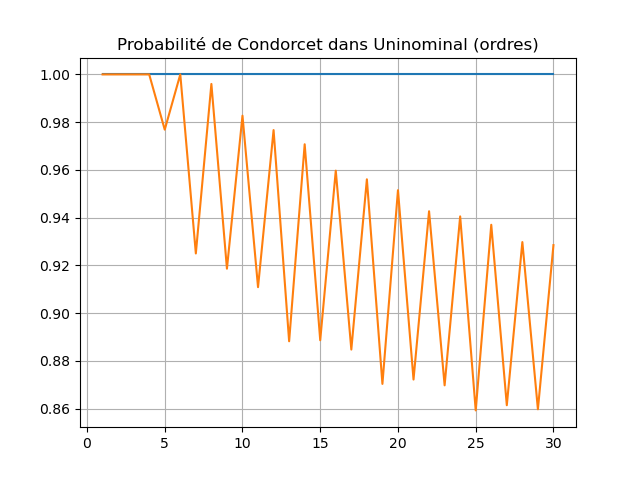
\includegraphics[scale=\sgh]{critereCondorcet/graphe_Uninominal_ordres_3_30.png}
		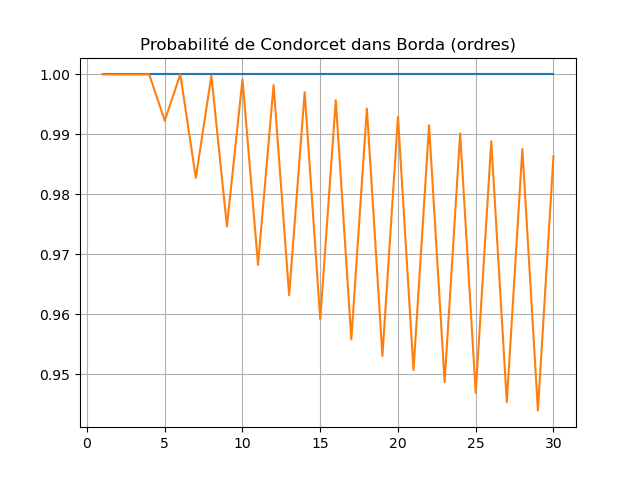
\includegraphics[scale=\sgh]{critereCondorcet/graphe_Borda_ordres_3_30.png}
	\end{frame}
	
	\begin{frame}{Critère d'honnêteté pour $\mathcal{D}_\mathcal{O} = \mathfrak{O}$}
		\def \sgh {0.29} % scale graphe
		
		
\includegraphics[scale=\sgh]{honnetete/graphe_Uninominal_ordres_3_30.png}
		
\includegraphics[scale=\sgh]{honnetete/graphe_Borda_ordres_3_30.png}
		
\includegraphics[scale=\sgh]{honnetete/graphe_Black_ordres_3_30.png}
		
\includegraphics[scale=\sgh]{honnetete/graphe_Copeland_ordres_3_30.png}
	\end{frame}
	
	\begin{frame}{Critère d'honnêteté pour $\mathcal{D}_\mathcal{O} = \mathcal{O}$}
		\def \sgh {0.29} % scale graphe
		
		\hspace{0.37\paperwidth}
		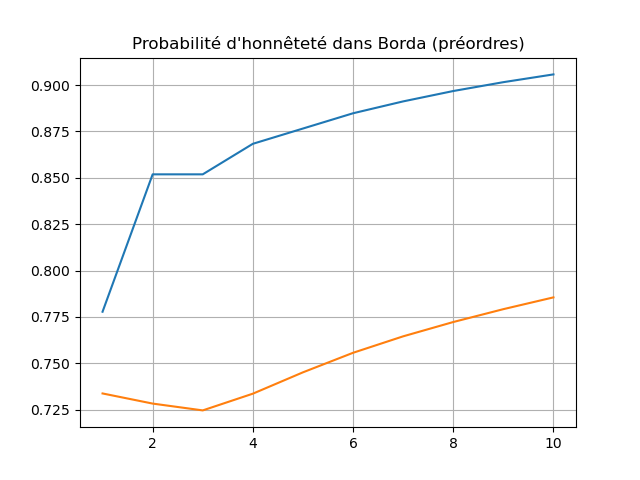
\includegraphics[scale=\sgh]{honnetete/graphe_Borda_préordres_3_10.png}
		
\includegraphics[scale=\sgh]{honnetete/graphe_Black_préordres_3_9.png}
		
\includegraphics[scale=\sgh]{honnetete/graphe_Copeland_préordres_3_9.png}
		%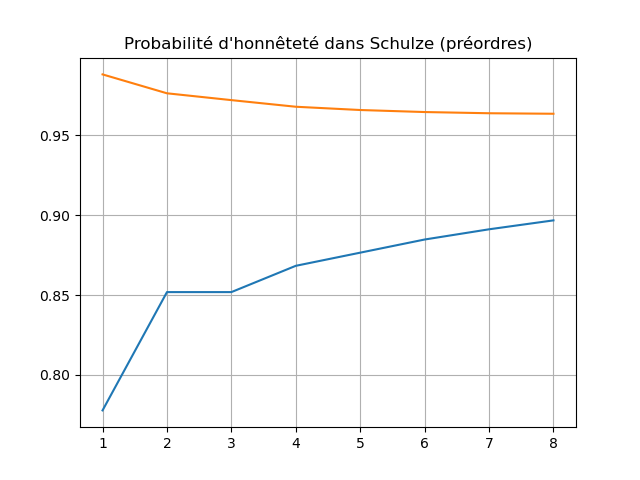
\includegraphics[scale=\sgh]{honnetete/graphe_Schulze_préordres_3_8.png}
	\end{frame}
	
	\section{Conclusion}
	\begin{frame}
		\begin{itemize}
			\uncover<1-6>{\item Méthode de Borda : fausse bonne idée}
			\uncover<2-6>{\item Scrutin uninominal : insatisfaisant}
			\uncover<3-6>{\item Méthode Black : préférable}
			\uncover<4-6>{\item Méthode de Copeland : selon le domaine de vote}
			%\uncover<5-6>{\item Méthode de Schulze : (étudiée dans le compte-rendu) la meilleure}
			% Dire à l'oral
		\end{itemize}
		\uncover<6>{Les relations d'ordre favorisent plus l'honnêteté que les relations de préordre.}
	\end{frame}
	
	\appendix
	\section{Annexes}
	
	\subsection{Unicité du vainqueur}
	\begin{frame}{Critère d'unicité du vainqueur pour $\mathcal{D}_\mathcal{O} = \mathfrak{O}$}
		\def \sgh {0.29} % scale graphe
		
		
\includegraphics[scale=\sgh]{unique_vainqueur/graphe_Uninominal_ordres_3_30.png}
		
\includegraphics[scale=\sgh]{unique_vainqueur/graphe_Borda_ordres_3_30.png}
		
\includegraphics[scale=\sgh]{unique_vainqueur/graphe_Black_ordres_3_30.png}
		
\includegraphics[scale=\sgh]{unique_vainqueur/graphe_Copeland_ordres_3_30.png}
	\end{frame}
	
	\begin{frame}{Critère d'unicité du vainqueur pour $\mathcal{D}_\mathcal{O} = \mathcal{O}$}
		\def \sgh {0.29} % scale graphe
		
		
\includegraphics[scale=\sgh]{unique_vainqueur/graphe_Borda_préordres_3_10.png}
		
\includegraphics[scale=\sgh]{unique_vainqueur/graphe_Black_préordres_3_9.png}
		
\includegraphics[scale=\sgh]{unique_vainqueur/graphe_Copeland_préordres_3_9.png}
		
\includegraphics[scale=\sgh]{unique_vainqueur/graphe_Schulze_préordres_3_8.png}
	\end{frame}
	
	\subsection{Quatre choix}
	
	\begin{frame}{Critère d'honnêteté pour $\mathcal{D}_\mathcal{O} = \mathcal{O}$ et 4 choix}
		\def \sgh {0.29} % scale graphe
		
		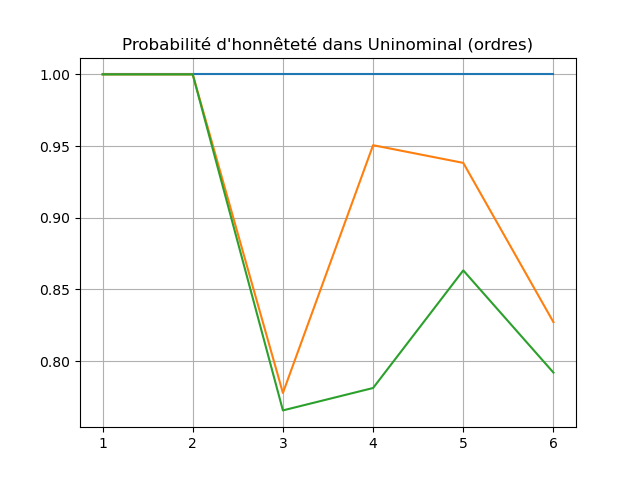
\includegraphics[scale=\sgh]{honnetete/graphe_Uninominal_ordres_4_6.png}
		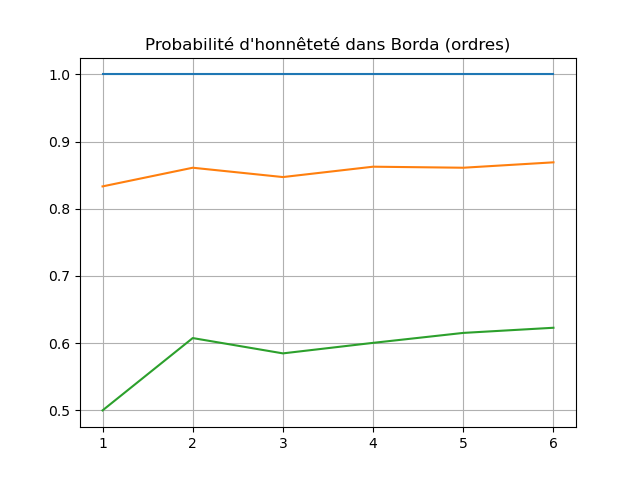
\includegraphics[scale=\sgh]{honnetete/graphe_Borda_ordres_4_6.png}
		
\includegraphics[scale=\sgh]{honnetete/graphe_Black_ordres_4_6.png}
		
\includegraphics[scale=\sgh]{honnetete/graphe_Copeland_ordres_4_6.png}
	\end{frame}
	
	\begin{frame}{Critère d'unicité du vainqueur pour $\mathcal{D}_\mathcal{O} = \mathcal{O}$ et 4 choix}
		\def \sgh {0.29} % scale graphe
		
		
\includegraphics[scale=\sgh]{unique_vainqueur/graphe_Uninominal_ordres_4_7.png}
		
\includegraphics[scale=\sgh]{unique_vainqueur/graphe_Borda_ordres_4_7.png}
		
\includegraphics[scale=\sgh]{unique_vainqueur/graphe_Black_ordres_4_6.png}
		
\includegraphics[scale=\sgh]{unique_vainqueur/graphe_Copeland_ordres_4_6.png}
	\end{frame}
	
	\subsection{Méthode de Schulze}
	\begin{frame}{Méthode de Schulze}
		\begin{tabular}{cc}
			\begin{tikzpicture}[
				node distance={3cm},
				thick,
				edge/.style = {draw, circle},
				arrow/.style={-{Stealth[length=4mm, width=3mm]}}
				]
				
				\node[edge, purple] (A) {A};
				\node[edge, purple] (B) [below left of=A] {B};
				\node[edge, purple] (C) [below right of=A] {C};
				\node[edge] (D) [below right of=B] {D};
				
				\draw[arrow, purple] (A) -- node[midway, above, sloped] {14} (B);
				\draw[arrow, purple] (B) -- node[near end, below, sloped] {10} (C);
				\draw[arrow, purple] (C) -- node[midway, above, sloped] {6} (A);
				\draw[arrow] (A) -- node[near end, above, sloped] {14} (D);
				\draw[arrow] (B) -- node[midway, above, sloped] {30} (D);
				\draw[arrow] (C) -- node[midway, above, sloped] {30} (D);
			\end{tikzpicture}
			&
			\begin{tikzpicture}[
				node distance={3cm},
				thick,
				edge/.style = {draw, circle},
				arrow/.style={-{Stealth[length=4mm, width=3mm]}}
				]
				
				\node[edge, purple] (A) {A};
				\node[edge, purple] (B) [below left of=A] {B};
				\node[edge, purple] (C) [below right of=A] {C};
				
				\draw[arrow, purple] (A) -- node[midway, above, sloped] {14} (B);
				\draw[arrow, purple] (B) -- node[near end, below, sloped] {10} (C);
				\draw[arrow] (C) -- node[midway, above, sloped] {6} (A);
			\end{tikzpicture}
		\end{tabular}
	\end{frame}
	
	\begin{frame}{Probabilité de critère pour la méthode de Schulze}
		\def \sgh {0.29} % scale graphe
		
		
\includegraphics[scale=\sgh]{honnetete/graphe_Schulze_ordres_3_25.png}
		
\includegraphics[scale=\sgh]{unique_vainqueur/graphe_Schulze_ordres_3_20.png}
		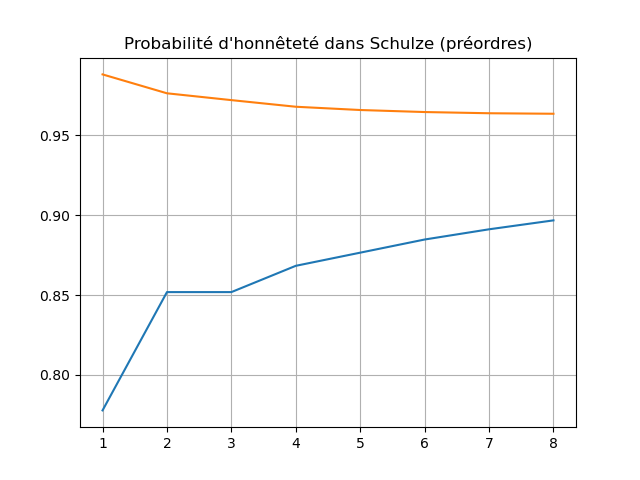
\includegraphics[scale=\sgh]{honnetete/graphe_Schulze_préordres_3_8.png}
		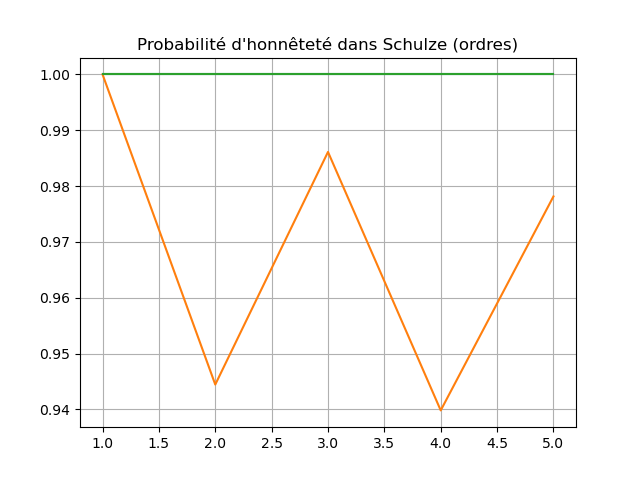
\includegraphics[scale=\sgh]{honnetete/graphe_Schulze_ordres_4_5.png}
	\end{frame}
\end{document}